%%====================================================================%%
%%                	AGH University of Science and Technology
%%	Faculty of Electrical Engineering, Automatics, IT and Electronics
%%			Department of Computer Science
%%				Master's thesis
%%
%%            Author : Adrian Wolny
%%        Speciality : Distributed systems and computer networks
%%      Register No. : 203789
%% Thesis Supervisor : Prof. dr hab. in�. Robert Schaefer
%%    Date (version) : 01.06.2011 0.1
%%
%%--------------------------------------------------------------------%%

\documentclass[pdflatex,11pt]{aghdpl}
%%\usepackage[polish]{babel}
\usepackage[utf8]{inputenc}
\usepackage{amsthm}
\usepackage{enumerate}
%%\usepackage{minted}
\usepackage{array}
\usepackage{algorithm}
\usepackage{algorithmic}
\usepackage{amsmath}
\usepackage{amsfonts}
\usepackage{listings}

\graphicspath{{./img/}}

\theoremstyle{definition}

\renewcommand{\topfraction}{0.85}
\renewcommand{\textfraction}{0.1}

\newtheorem*{definition}{Definition}
%%\newtheorem{przyklad}{Przyk�ad}

%%\newminted{java}{gobble=4, linenos, numbersep=8pt}
%%\newminted{js}{gobble=4, linenos, numbersep=8pt}
%%\newminted{xml}{gobble=4, linenos, numbersep=8pt}
%%\renewcommand{\theFancyVerbLine}{\ttfamily\small\oldstylenums{\arabic{FancyVerbLine}}}

%---------------------------------------------------------------------------

\author{Adrian Wolny}

%%\titlePL{Poprawa algoryt�w populacyjnych w problemach optymalizacji globalnej
%%poprzez deterioracj� funkcji przystosowania}
\titleEN{Improving population-based algorithms used in Global Optimization with
Fitness Deterioration techniques}

%%\thesistypePL{Praca magisterska}
\thesistypeEN{Master of Science Thesis}

%%\supervisorPL{Prof. dr hab. in�. Robert Schaefer}
\supervisorEN{Robert Schaefer, Prof., PhD, DSc}

\date{2011}

%%\departmentPL{Katedra Informatyki}
\departmentEN{Department of Computer Science}

%%\facultyPL{Wydzia� Elektrotechniki, Automatyki, Informatyki i Elektroniki}
\facultyEN{Faculty of Electrical Engineering, Automatics, Computer Science and Electronics}

\acknowledgements{\ldots}

\setlength{\cftsecnumwidth}{10mm}

%---------------------------------------------------------------------------

\begin{document}


\chapter{Fitness Deterioration}
\label{ch:fitnessDet}

This chapter contains detailed description of the deterioration algorithm
which is the central point of the \textit{Cluster Supported Fitness
Deterioration} algorithm described in chapter \ref{ch:csfdAlgorithm}. 
Before diving into the details, here is the formal definition of the fitness
deterioration process:
\textit{Fitness Deterioration} is a process of degrading the fitness
function in areas occupied by groups of individuals obtained from
clustering (see Section \ref{sec:Fdt} and references inside). 
We suggest to achieve this goal in the CSFD strategy by creating a linear combination 
of the current fitness function and \textit{crunching functions} which approximate
the fitness in subsets of problem domain occupied by clusters.
Let $F_k$ be the fitness function in $k$-th iteration of CSFD
(i.e. in the $k$-th execution of the main loop of the Algorithm \ref{alg:CSFD})
and $C_1, \ldots, C_{M_k}$ be
$M_k$ clusters found in $k$-th iteration of our new sequential niching algorithm 
(algorithm \ref{alg:CSFD} described in Section \ref{sec:algDesc}).
For each cluster $C_i$ we create the \textit{crunching function} $g_i$ and then
we construct deteriorated fitness $F_{k+1}$ (which will be used in the
$(k+1)$-th iteration) as follows:

\begin{equation}
\label{eqn:fitDet}
F_{k+1} = F_k + \sum_{i=1}^{M_k} \alpha_i g_i,
\end{equation}
where the selection of the functional coefficients 
$\alpha_1, \ldots, \alpha_{M_k}; \; \alpha_i:\mathcal{D} \rightarrow \mathbb{R}_+, \,
i = 1, \ldots, M_k$ depends on the
type of deterioration used and will be described later in Sections
\ref{sec:BasScheme}, \ref{sec:WeightScheme}
(see formulas (\ref{eqn:alpha1}), (\ref{eqn:alpha2}), 
(\ref{eqn:fractures})).
 

The \textit{Crunching function} $g_i: \mathcal{D} \rightarrow \mathbb{R}_+$ 
is constructed for each newly recognized cluster of individuals
$C_i \subset P$.
Based on the assumption that clusters lie inside basins
of attraction and that the distribution of individuals inside the cluster
is a good approximation of the shape of the basin occupied by the cluster,
the deterioration algorithm tries to exploit information
provided by the clustering algorithm and based 
on that information it augments the fitness function in order to minimize 
the probability of finding already explored basins of attraction in further iterations.

We may ask ourselves why we do not prevent exploration of basins 
we found in previous iterations simply by remembering the regions occupied
by clusters and ignoring individuals which fall in this regions.
The answer is probably the most important reason why we have chosen fitness
deterioration for this task. 
We can not prevent individuals to explore
neighborhood of solutions found in previous iterations because such
approach would cause our meta-heuristic to loose \textit{completeness} (see
\cite{PardalosRomeijn2002}).

\begin{definition}\label{completeness}
A set $Op$ of search operations searchOp is \textit{complete}
if and only if every point $g_1$ in the search space \mathbb{G}
can be reached from every other point $g_2 \in \mathbb{G}$ by applying
only operations $searchOp \in Op$.
\begin{equation}
\forall g_1, g_2 \in \mathbb{G} \Rightarrow \exists k \in \mathbb{N}:
P(g_1=Op^k(g_2)) > 0
\end{equation} 
\end{definition}

If the set of search operations is not complete, there are points 
in the search space which cannot be reached. 
Then, we are probably not able to explore the problem space adequately 
and possibly will not find satisfyingly good solution. 
That is why it is better to use fitness deterioration as a way to discourage
rather then prevent individuals from sinking to the same basins of attraction twice.

Here we would like to emphasize the fact that the
deterioration process does not try to accurately interpolate the fitness
function in the neighborhood of the solution because it would be very
expensive in a high dimensional spaces. Instead it tries to find simple
crunching functions which would sufficiently degrade the fitness landscape in the areas 
occupied by the clusters and then remove the individuals from these regions
in the next CSFD steps with the sufficiently high (but even less then 1) probability.


We now can define what are the characteristics of a good deterioration
algorithm:
\begin{itemize}
  \item \textit{It has to be chep} in terms of space and time. We are looking
  for methods which can be successfully applied for solving high
  dimensional functions' optimization. After every iteration the resulting
  fitness function is the linear combination of crunching functions, therefor we
  must ensure that computation of a single crunching function is $O(1)$ and does 
  not depend no the number of individuals inside a cluster or the number of
  clusters. Resulting fitness must be $O(k)$ where $k$ is the number of
  solutions (clusters) found in previous iterations.
  
  \item \textit{It has to discourage the population of EA from visiting the
  neighborhood of solutions found in previous iterations twice}. We do not want
  these regions to be inaccessible as this would break the \textbf{completeness} 
  of our algorithm, we just want an individual to be given a low fitness when it
  finds itself in these regions.
  
  \item \textit{It has to be easy to extend for subsequent solutions}. The way
  we construct fitness function in subsequent iterations already fulfills
  this requirement. To extend the deterioration for subsequent solutions we
  simply add new crunching functions multiplied by the scaling factors we define
  later in this chapter. 
\end{itemize}


\begin{definition}\label{premature-convergence}
\textit{Premature Convergence} \cite{PardalosRomeijn2002} An optimization process has
\textit{prematurely converged} to a local optimum if it is no longer able to explore 
other parts of the search space than the area currently being examined and there 
exists another region that contains a superior solution.
\end{definition}

The premature convergence is not a problem in our algorithm, because once the
population finds itself in the local optima trap it is very likely that the
population will be avoiding this region in the next iterations. Actually we
encourage an optimization process performed by the used EA (e.g. SGA) 
to converge quickly to local solution in order to find new solutions 
faster in the next iterations. 

An ideal GA engine to be used in our hybrid algorithm defined in Section
\ref{sec:algDesc} would be the one which produces many small populations in problem space and
each population would use strong selection pressure with small mutation rate
with high recombination rate to increase exploitation. This is why Hierarchical 
Genetical Search (HGS) \cite{WierzbaSemczukKolodziejSchaefer2003} algorithm
would be perfect for our needs as it possess all of the listed characteristics. 
However we may also choose some simple 
SGA or Evolution Strategy with small population size and strong exploitation
characteristics.
 

\section{Fitness deterioration and clustering}
\label{sec:FitDetClust}

To increase the accuracy of the fitness deterioration process 
we want to use the maximum amount of information provided by the clustering
algorithm. As we mentioned at the begining of this chapter we create one
crunching function per cluster which, depending on the shape of the cluster, 
may not be very accurate or may even degrade areas
of the fitness landscape which have not been explored yet and potentially
contain valuable solutions. 
Figure \ref{fig:hardClusters1} shows cases in which
crunching functions created for extracted clusters strongly affect regions outside the clusters.

\begin{figure}
  \centering
  \fbox{
    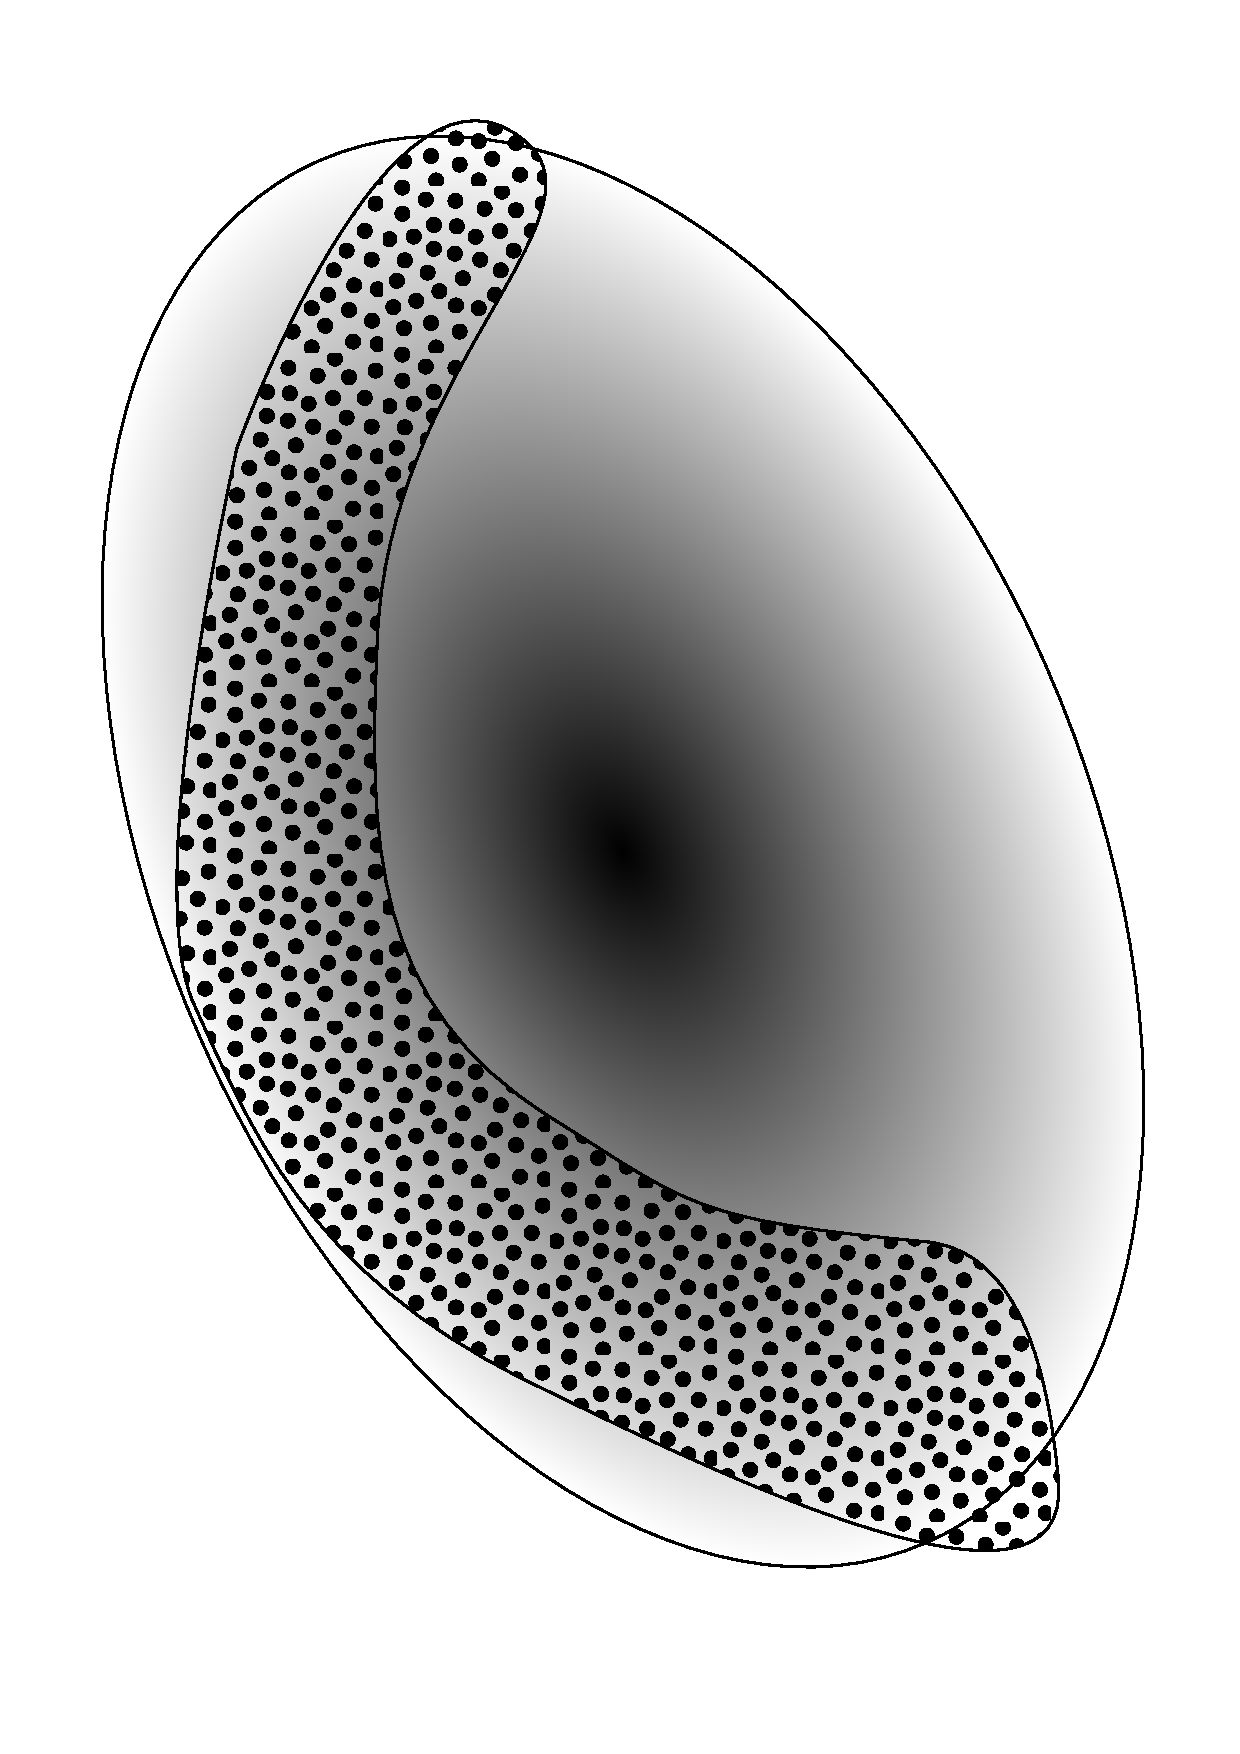
\includegraphics[scale=0.15]{clusterDensity/hardcluster1.pdf}
  }
  \fbox{
    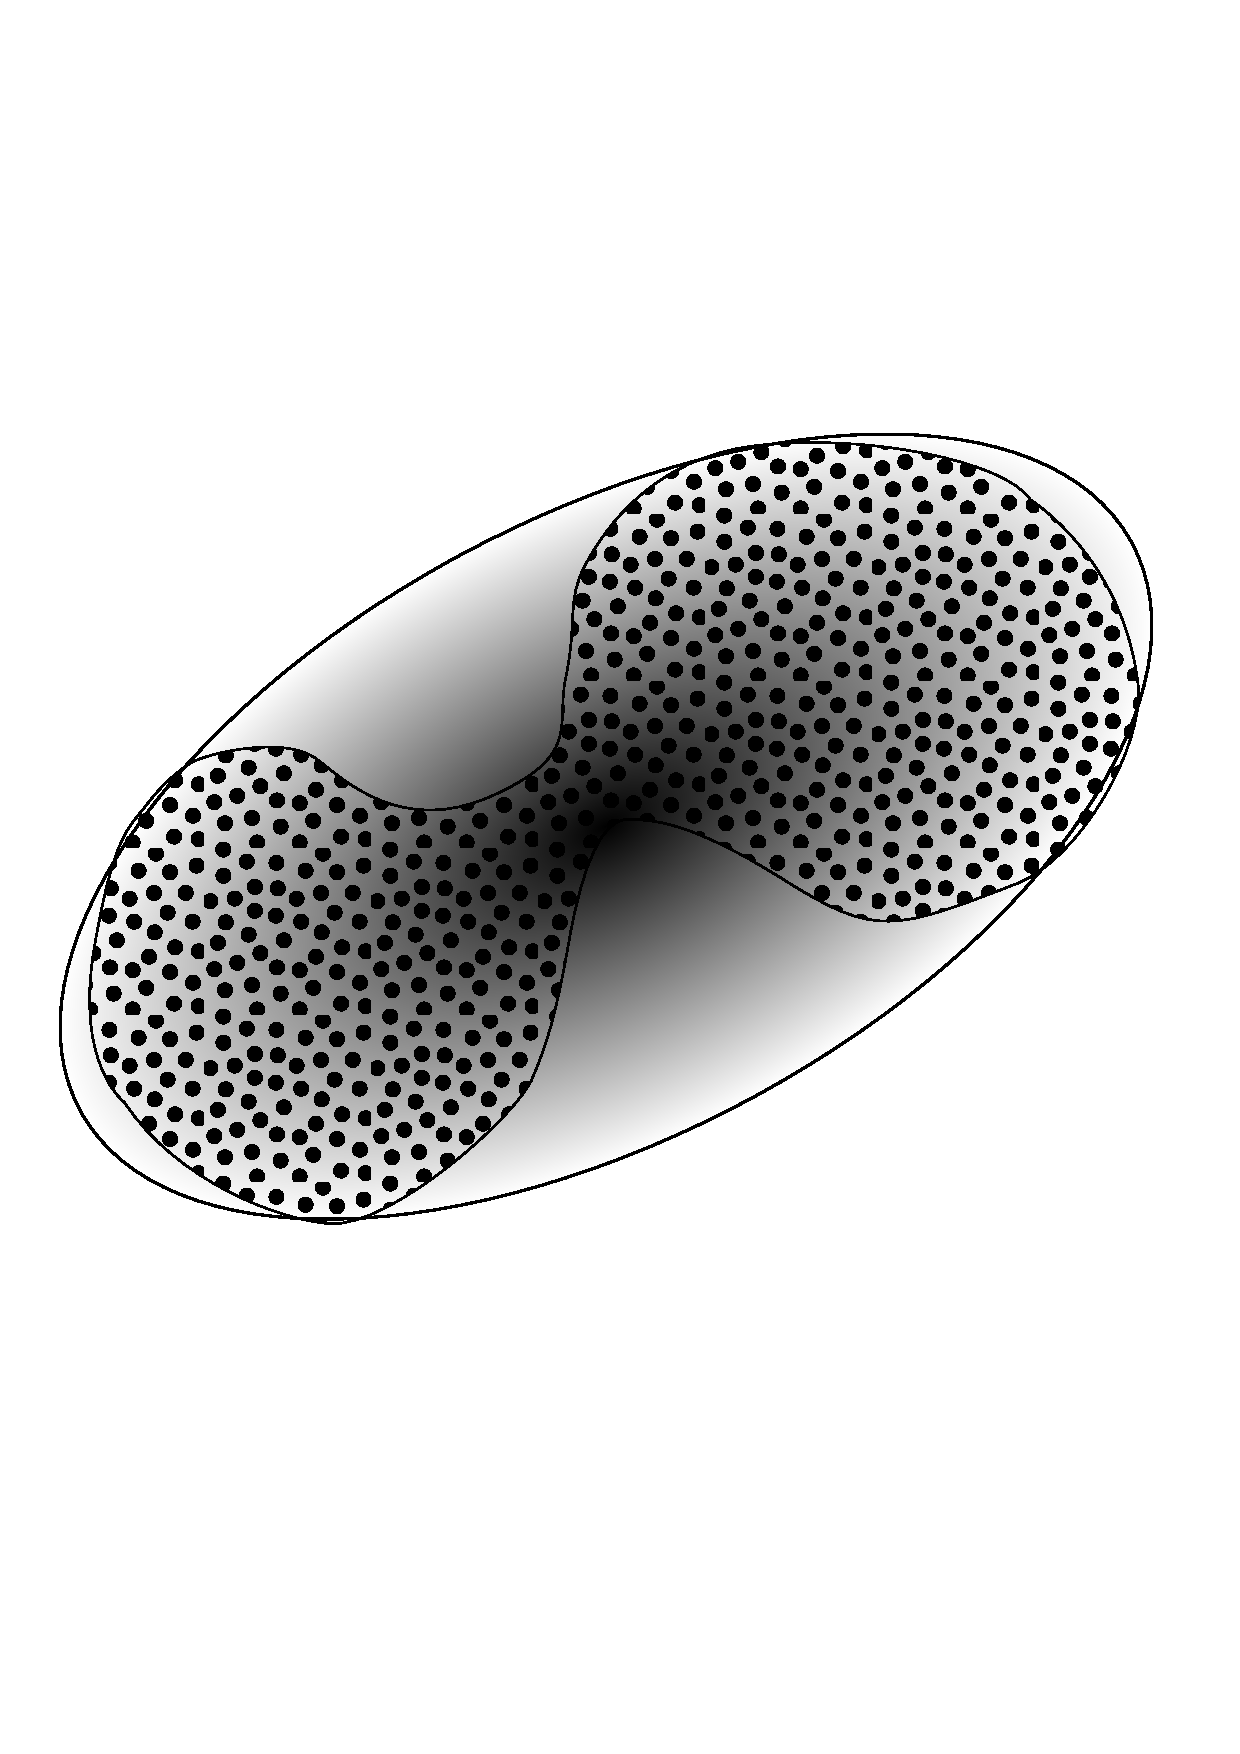
\includegraphics[scale=0.15]{clusterDensity/hardcluster2.pdf}
  }
  \caption{Example of two clusters returned by the clustering algorithm
  and corresponding Gaussian \textit{crunching functions} which degrade
  areas distant from clusters.}
  \label{fig:hardClusters1}
\end{figure}
 
 
To increase the accuracy of our algorithm
we use the following property of the OPTICS \textit{ordering}:
\begin{quotation}
\noindent
While creating the ordering, OPTICS constructs density-based clusters
with respect to different densities simultaneously. OPTICS ordering
actually contains the information about the intrinsic clustering structure of
the input data set (up to the generating distance $\epsilon$) 
(see \cite{optics}).
\end{quotation}

This might be shown for sample data (see Figure \ref{fig:opticsOrder1}) by using its
\textit{reachability plot}. Once we create OPTICS ordering
we may easily extract clusters with higher densities by decreasing
$\epsilon$ and choose clusters for which MSE (Mean--Square Error) 
between the actual fitness function and the crunching function in the 
areas of clusters is minimal.

The algorithm works as follows (see Algorithm \ref{alg:IFDA}): 
having the OPTICS ordering
of the population returned by the EA our method iteratively extracts 
clusters with higher densities by decreasing the \textit{neighborhood radius $\epsilon$} 
(see Figure \ref{fig:opticsOrder2}), and then by constructing crunching
function for extracted clusters and checking if the resulting crunching functions is more accurate than the best found in previous iterations (MSE comparison).

\begin{algorithm}
\caption{Improving fitness deterioration accuracy}
\label{alg:IFDA}
\begin{algorithmic}[1]
\STATE {$\epsilon'=\epsilon$}
\WHILE{$\epsilon' > treshold$}
	\STATE {$cs \leftarrow extractDBSCANClustering(\epsilon')$}
	\STATE {$crunchFs \leftarrow createCrunchingFunctions(cs)$}
	\STATE {$mse \leftarrow getMSE(crunchFs, currentFitness, cs)$}
	\IF{$mse < minMSE$}
		\STATE {$saveBestCrunching(mse, crunchFs)$}
	\ENDIF
	\STATE {$\epsilon' \leftarrow \epsilon' * 0.8$}
\ENDWHILE
\end{algorithmic}
\end{algorithm}

Algorithm \ref{alg:IFDA} effectively prevents the deterioration process
from destroying the fitness landscape in regions not yet explored by
the CSFD algorithm. 
Figure \ref{fig:hardClusters2} shows how the $\epsilon$
adjustment can improve the shape of the cluster extension
with respect to the initial one (see Figure \ref{fig:hardClusters1}).
To better understand how do we 
use OPTICS ordering to extract cluster of higher density see
Figures \ref{fig:opticsOrder1} and \ref{fig:opticsOrder2}.

\begin{figure}
  \centering
  \fbox{
    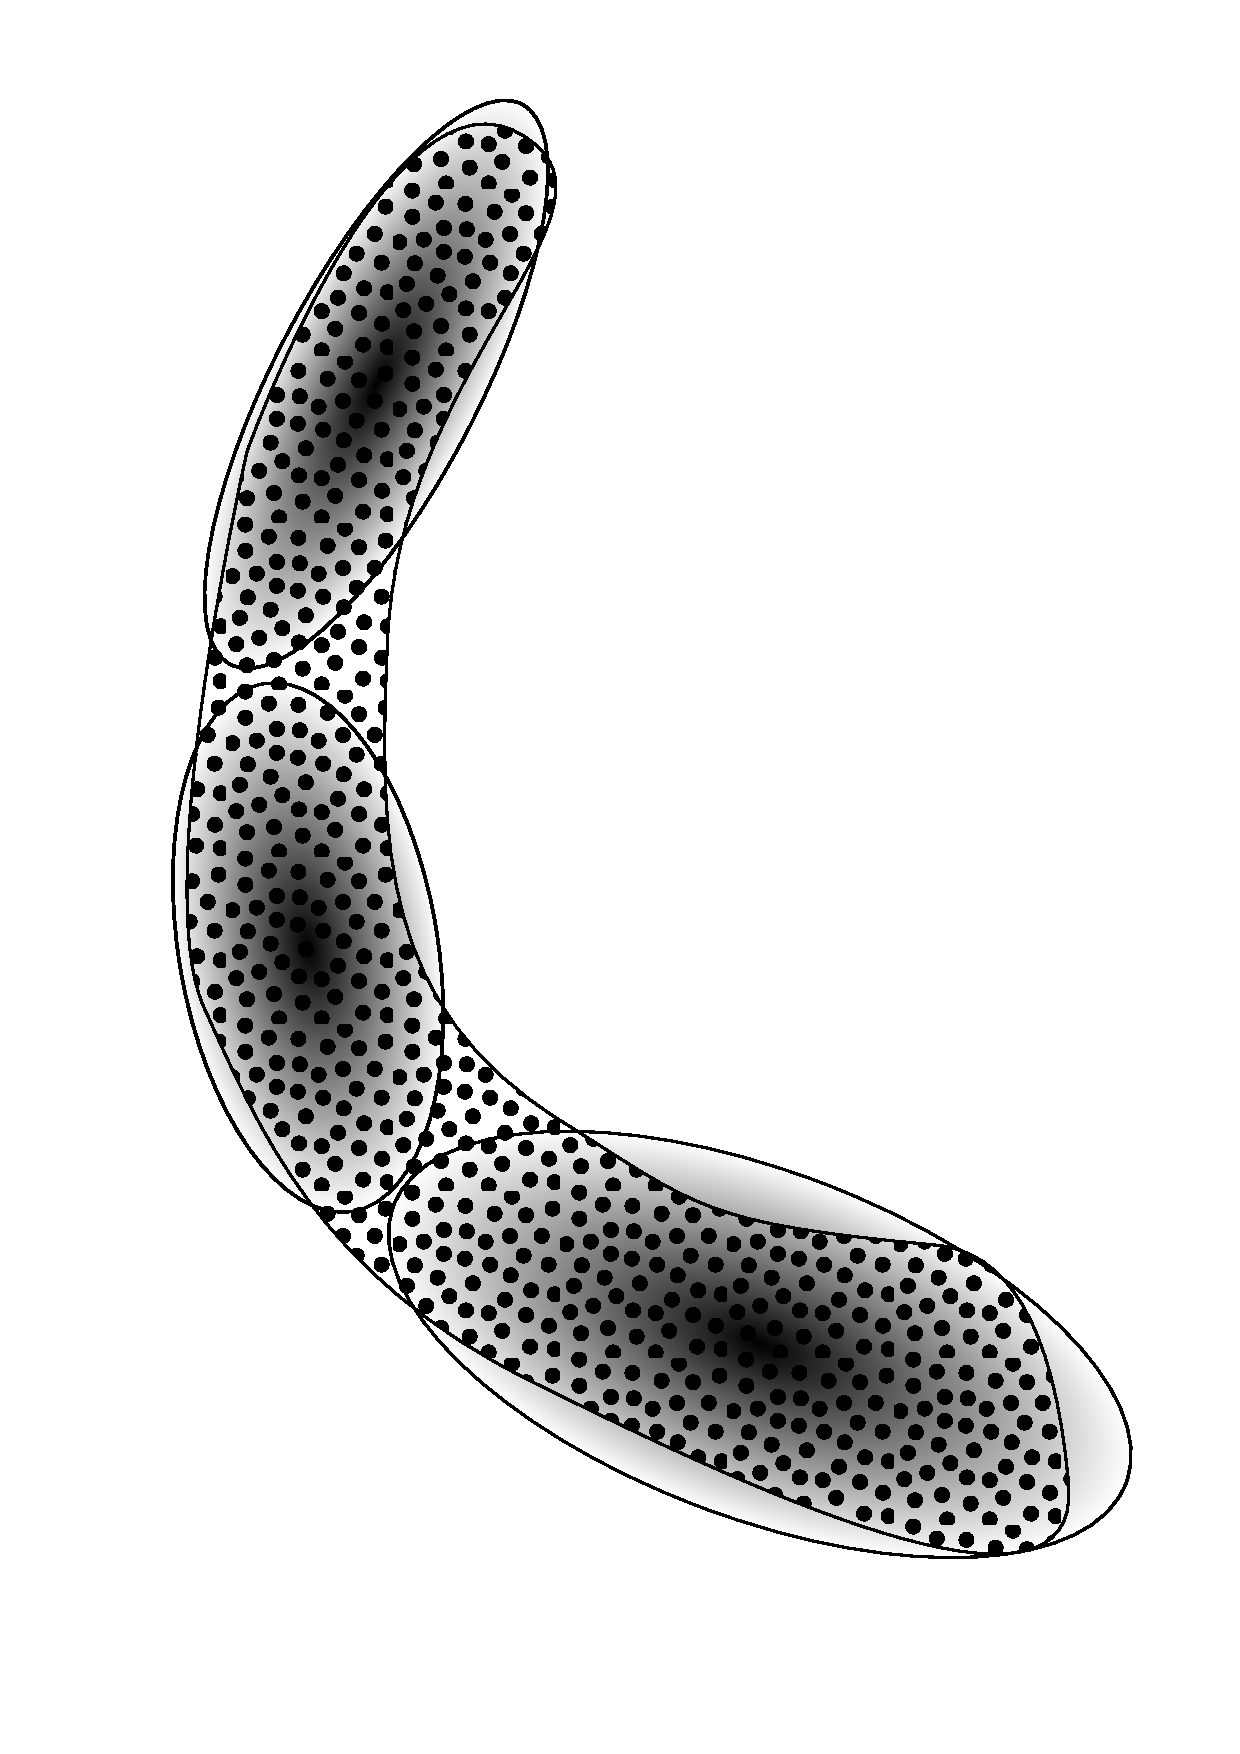
\includegraphics[scale=0.15]{clusterDensity/hardcluster12.pdf}
  }
  \fbox{
    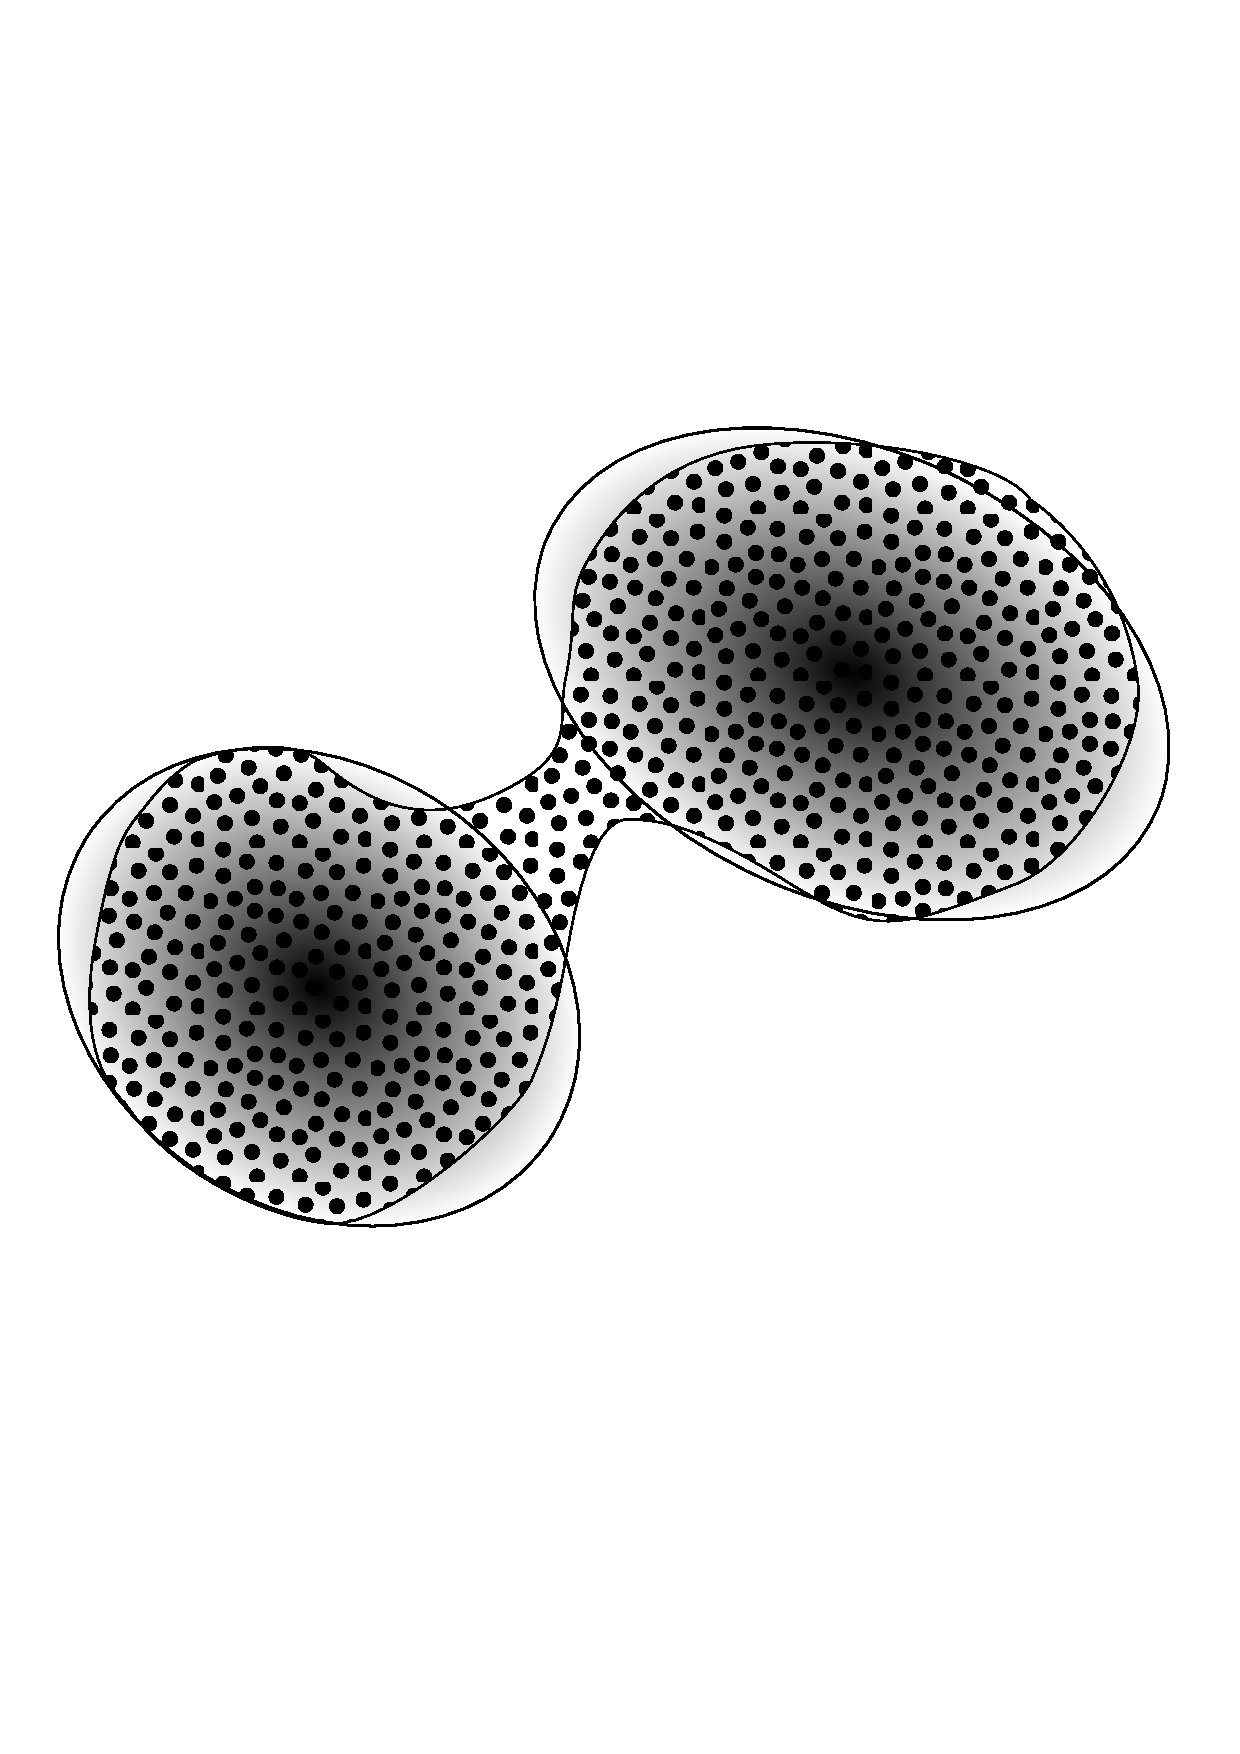
\includegraphics[scale=0.15]{clusterDensity/hardcluster22.pdf}
  }
  \caption{With \textit{OPTICS ordering} we may extract cluster of higher
  densities and minimize the impact of the fitness deterioration on regions
  outside the clusters (instead of creating one crunching function per cluster 
  like in figure \ref{fig:hardClusters1} we extract denser clusters from the
  \textit{ordering} and create crunching function which degrade only 
  the region occupied by the cluster)}
  \label{fig:hardClusters2}
\end{figure}



\begin{figure}
  \centering
  \fbox{
    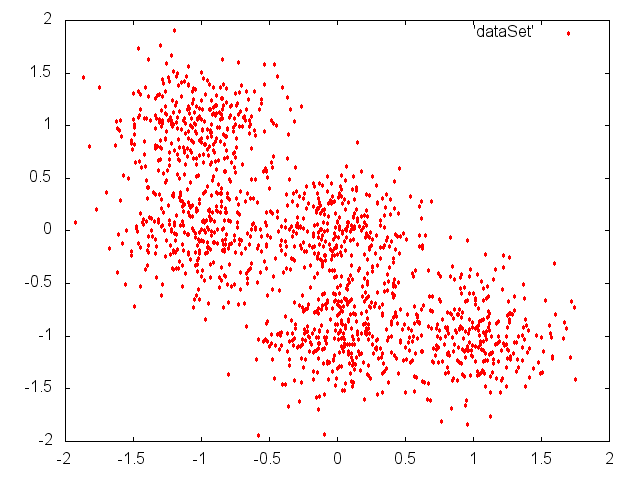
\includegraphics[scale=0.3]{clusterExtraction/extDataSet.png}
  }
  \fbox{
    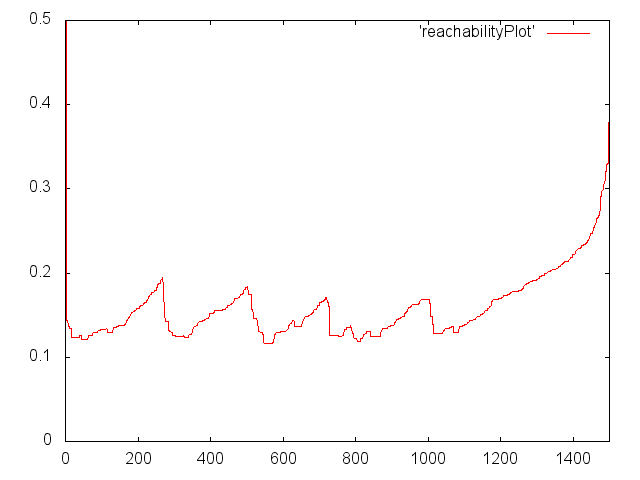
\includegraphics[scale=0.4]{clusterExtraction/reachabilityPlot.png}
  }
  \caption{Sample data set of 1500 points and the corresponding reachability plot
  of the ordered points (shows the reachability distance of each individual in the
  data set - horizontal axis corresponds to the individuals in the data set and
  the vertical axis shows the reachability distance of a given individual)
  OPITCS ordering parameters: $\epsilon=1.0$ $minPts=30$. 
  Cavities in the plot depict 5 clusters which might be extracted from the data
  set by the DBSCAN algorithm using proper value of $\epsilon'$ values}
  \label{fig:opticsOrder1}
\end{figure}

\begin{figure}
  \centering
  \fbox{
    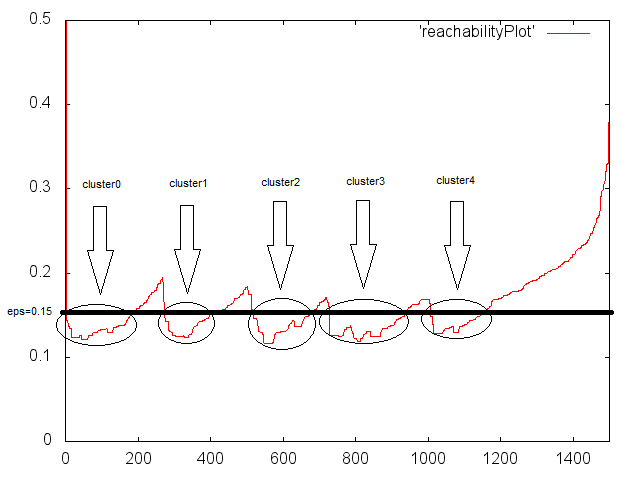
\includegraphics[scale=0.4]{clusterExtraction/reachabilityPlot1.png}
  }
  \fbox{
    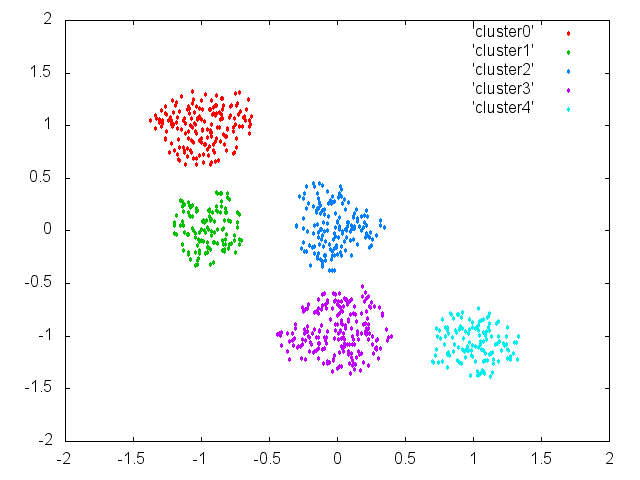
\includegraphics[scale=0.3]{clusterExtraction/extClusters.png}
  }
  \caption{Extraction of clusters from the data set presented in Figure
  \ref{fig:opticsOrder1} using DBSCAN algorithm with 
  $\epsilon'=0.15$. The value of $\epsilon'$ is marked on the first
  plot which shows reachability distances and the "cut off" clusters}
  \label{fig:opticsOrder2}
\end{figure}
 


\section{Basic Scheme}
\label{sec:BasScheme}

The basic version of our deterioration algorithm is as follows.
For each cluster $C$ generate a multi-dimensional Gaussian function
$g: V \rightarrow \mathbb{R}_+$
\begin{equation}
\label{eqn:GF}
g(x)= F_k(x_{max}) \,  exp \left(
 - \frac{1}{2}(x - \overline{m})^T \, \Sigma^{-1} \, (x - \overline{m})
\right)
\end{equation}
where $F_k$ is the fitness function in $k$-th iteration of the CSFD algorithm,
$x_{max}$ is the fittest individual from the cluster, the $\overline{m}$ is the
cluster's centroid (mean phenotype of invividuals belonging to $C$)
and $\Sigma$ is unbiased sample covariance matrix
estimated from the cluster population by the formula (\ref{eqn:Sigma})
(see e.g. \cite{SampleCovariance})
\begin{equation}
\label{eqn:Sigma}
\Sigma = \frac{1}{Card(C) - 1} \, \sum_{x \in C} 
(x - \overline{m}) \otimes (x - \overline{m})
\end{equation}
where $\otimes$ stands for the tensor product symbol. Please, notice, that
the sum in (\ref{eqn:Sigma}) is spanned over all individuals belonging
to the cluster $C$ i.e. the phenotype $x$ might be counted more than once,
if is repeatedly represented in $C$.


Fitness function in the $(k+1)$-th iteration is obtained from the equation
(\ref{eqn:fitDet}) by seting $\alpha_i \equiv 0, \, i = 1,\ldots,M_k$.



Big advantage of this algorithm are simplicity and speed.
However, this version may cause strong deformation of the
fitness landscape in areas which are distant from the already found clusters,
which is unacceptable. To overcome this issue we
developed so called \textit{weighted scheme} described 
in the next Section \ref{sec:WeightScheme}. 





\section{Weighted Scheme}
\label{sec:WeightScheme}

This type of fitness deterioration is more accurate and is likely to produce
more stable fitness that basic scheme, cause the latter may produce
sharp peaks in the fitness landscape, because of the very aggressive fitness degeneration.
Weighted Scheme is also more complex cause it generates
more computationally intensive fitness functions.

Initial steps are the same as in basic scheme, we create 
multi-dimensional Gaussian function for each cluster. 
What is different is how we compute the new (deteriorated) 
fitness is the following way
\begin{equation}
\label{eqn:WS1}
F_{k+1}(x) = F_k(x) + \sum_{i=1}^{M_k} \alpha_i(x) g_i(x),
\end{equation}
where the $\alpha$-coefficients are given by the following equations
\begin{equation}
\label{eqn:alpha1}
\alpha_1(x) \, +, \ldots, + \, \alpha_{M_k}(x) = 1,
\end{equation}
\begin{equation}
\label{eqn:alpha2}
\alpha_i(x) = \xi(x) \, \left( \frac{1}{r_i(x)} \right),
\end{equation}
\begin{equation}
\label{eqn:fractures}
\frac{1}{\xi(x)} = \frac{1}{r_1(x)} \, +, \ldots, + \, \frac{1}{r_{M_k}(x)},
\end{equation}
where $r_i(x) = \left\| x - \overline{m}_i \right\|$ is the distance between $x$ 
and the $C_i$ centeroid $\overline{m}_i$ (see Figure \ref{fig:weightedScheme}). 
So in order to compute fitness for a 
given individual $x$ (more correctly for $ph(x)$) 
we have firstly compute distances $r_i(x)$. 
Then we compute $\xi(x)$ from the equation (\ref{eqn:fractures}), next the
$\alpha$-coefficients from the system (\ref{eqn:alpha1}),(\ref{eqn:alpha2})
and finally the fitness value from (\ref{eqn:WS1}).
$\alpha$-coefficients are computed separately for each new individual 
and this is why this method is more costly than the previous one.
\begin{figure}
  \centering
  \fbox{
    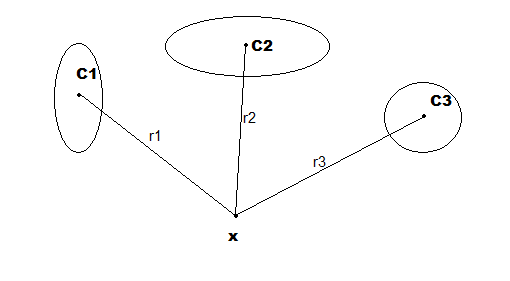
\includegraphics[scale=0.4]{AdaptiveScheme.png}
  }
  \caption{The coefficient $\alpha_i$ is inversely proportional to the 
  distance from the center of cluster $C_i$ to the $x$. $\alpha_i$ may
  be seen as the impact $C_i$ has on $x$}
  \label{fig:weightedScheme}
\end{figure}
From the equations (\ref{eqn:WS1})-(\ref{eqn:fractures}) 
it is clear that regions of domain
which are distant from clusters found in previous iterations of the algorithm
are very little affected by the crunching functions which is a big advantage
over the basic scheme. 
However, experiments shows that the basic
scheme yields very good results and is preferable over the weighted
scheme due to the lower computational cost of the former.



\section{Crunching Function Adjustment}
\label{sec:CrumchAdj}


Because of the fast convergence of populations
generated by the GA algorithm to the local solutions 
and the features of the Algorithm \ref{alg:IFDA} used
to increase accuracy of the deterioration process, %(see Section \ref{sec:OPTICS}),
clusters sometimes become very dense in areas close to the local minimizers. 
Gaussians created for such
clusters does not approximate a basin of attraction well, speaking informally:
Gaussian functions created for such clusters consist of high and thin peaks
which deteriorate only the area inside the cluster, 
only the narrow basin of attraction
in which the cluster resides.
To overcome this issue we developed so called \textit{Crunching Function
Adjustment} (CFA) algorithm described below.


We use sample covariance matrix as an estimator (see \cite{SampleCovariance}), which
is extremely sensitive to outliers. However we may take this property as our
advantage and incorporate it CFA algorithm. 
Having given a cluster of points the CFA algorithms works as follows:

\begin{itemize}

  \item We estimate the covariance matrix $\Sigma$ 
  and then compute its $N$ eigenvectors
  ($N = dim(V)$ is the dimension of the problem space). 
  They are ortogonal one to each other
  and define the orientation of the Gaussian "bell"
  
  \item for each eigenvector $v_i$ we generate two points 
  $\underline{p_i}, \overline{p_i}$ called \textit{leading marks}
  \begin{eqnarray}
  \label{eqn:outliners}
  \overline{p_i} = \overline{m} + \sqrt{\lambda_i} \, v_i \nonumber\\
  \underline{p_i} = \overline{m} - \sqrt{\lambda_i}\, v_i
  \end{eqnarray} 
  where $\overline{m} \in V$ is the cluster's centroid and $\lambda_i$ is
  an eigenvalue of the eigenvector $v_i$.
  
  \item Then we add these $2 N$ generated leading marks to the initial
  multiset which constitute a cluster, and compute new covariance matrix.
  
  \item Because the sample covariance matrix is very sensitive to leading marks,
  the resulting covariance matrix produces a Gaussian function whose "bell
  hypersurface" is more stretched in directions of eigenvectors.
  
  \end{itemize}
  
Please notice, that the improvement introduced above is purely heuristic,
having no precise mathematical motivation. It was designed only
for deterioration performed by Gauss functions and positively verified for
2D benchmarks (see Section \ref{sec:testFun}) so its usefulness 
in other cases in unknown.

\subsection{CFA Results}

The figures below shows the result of our CSFD algorithm with CFA for two
simple functions from $f:\mathbb{R}^2 \rightarrow \mathbb{R}$, specifically:
\begin{itemize}
  \item $f(X) = 2e^{-(x^2 + y^2)}$, where $X \in \mathbb{R}^2$
  \item $f(X) = e^{-(x^2 + y^2)}+1.4e^{-((x-1.7)^2 + (y-1.7)^2)}$, where $X \in
  \mathbb{R}^2$
\end{itemize}

\begin{table}[ht]
    \caption{The results of basic deterioration scheme applied to functions 
    $f(X) = 2e^{-(x^2 +y^2)}$ (up-left and down-left) and $f(X) = e^{-(x^2 +
    y^2)}+1.4e^{-((x-1.7)^2 + (y-1.7)^2)}$ (up-right and down-right) with the
    populations generated with normal distribution around the solutions. For
    the fist function we may see that the 
  	overall landscape decreases only by $30\%$ (down-left), while using
  	CFA gives us $85\%$ of decline (up-left). For the second function we
  	see $25\%$ of deterioration (down-right), while CFA gives us $78\%$
  	(up-right)}
    \centering
    \begin{tabular}{cc}
    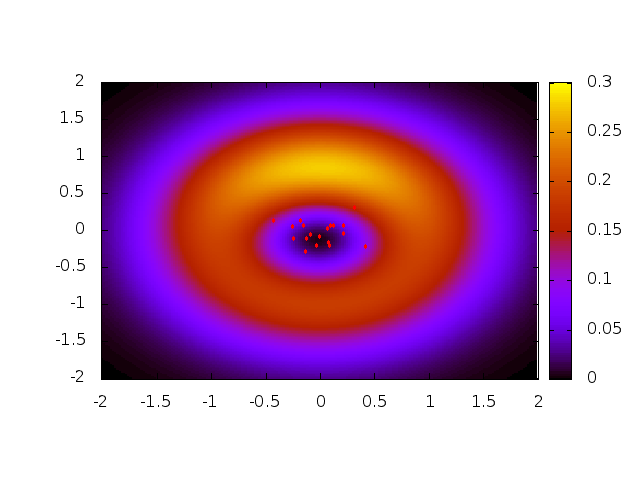
\includegraphics[scale=0.3]{CMA/result1_CMA.png} &
    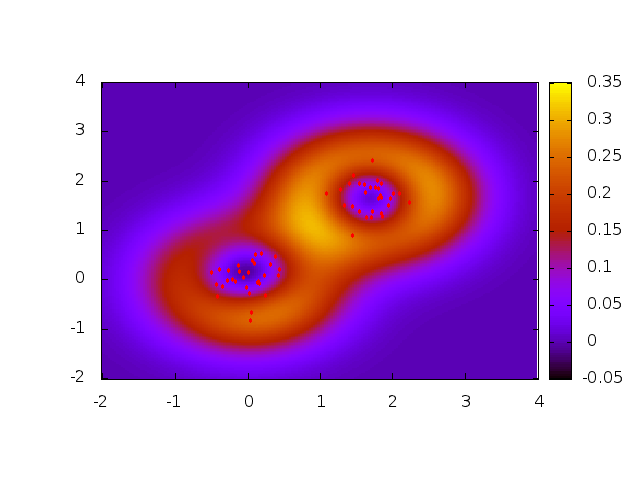
\includegraphics[scale=0.3]{CMA/result2_CMA.png} \\
    \newline
    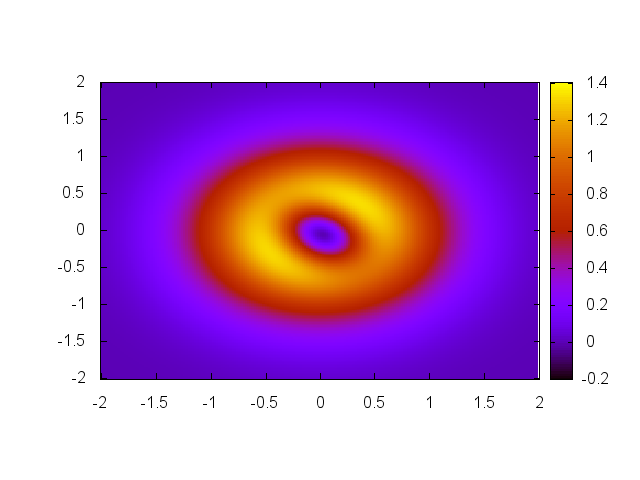
\includegraphics[scale=0.3]{CMA/result1_noCMA.png} &
    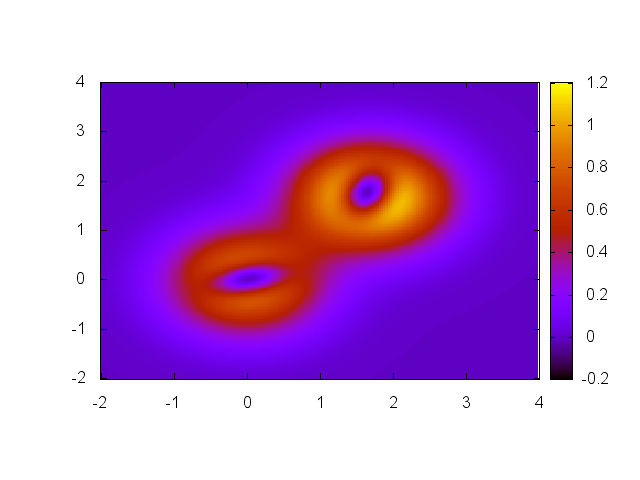
\includegraphics[scale=0.3]{CMA/result2_noCMA.png} \\
    \end{tabular}
    \label{tab:cfa}
\end{table}%

Table \ref{tab:cfa} shows how much the algorithm benefit
from using the CFA algorithm.

\bibliographystyle{alpha}

\end{document}
